\section{Data's distribution}

The dataset is composed of 70k .wav files which are already split ( training set : 58252 , validation set : 6137 , test set : 6231 ). Those files are regrouped in 30 differents words that can be learned. You can also find 6 extra files of differents length which are just common noises.


\begin{figure}[!h]
    \centering
    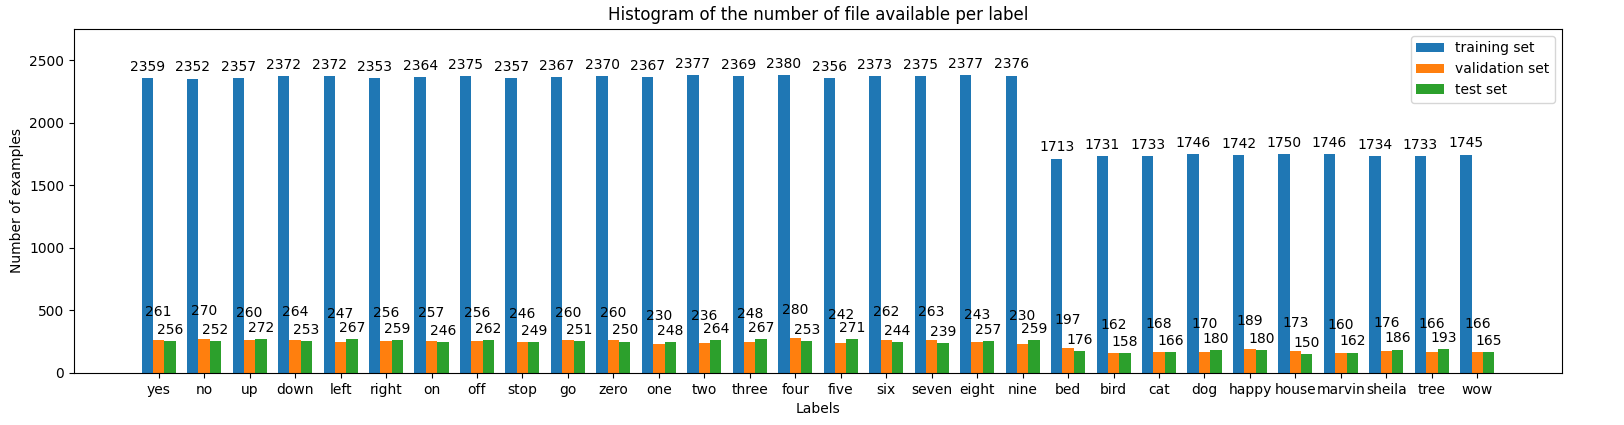
\includegraphics[width=1\textwidth]{chapters/pictures/histo_all.PNG}
    \caption{Files distributions}
    \label{fig:init_dist}
\end{figure}


Each file is supposed to contain a one second clip recorded at a rate of 16kHz. Therefore we should expect 16000 points once the file is loaded, but plenty of them are actually not one second long. This will bring problems later on since we need the inputs to be always the same length. We can either expend those data to get the same length as the others ( zero-padding, averaging, ...), we can cut the silences out of every file and take only the voices, or we can simply ignore them.



\begin{figure}[!h]
    \centering
    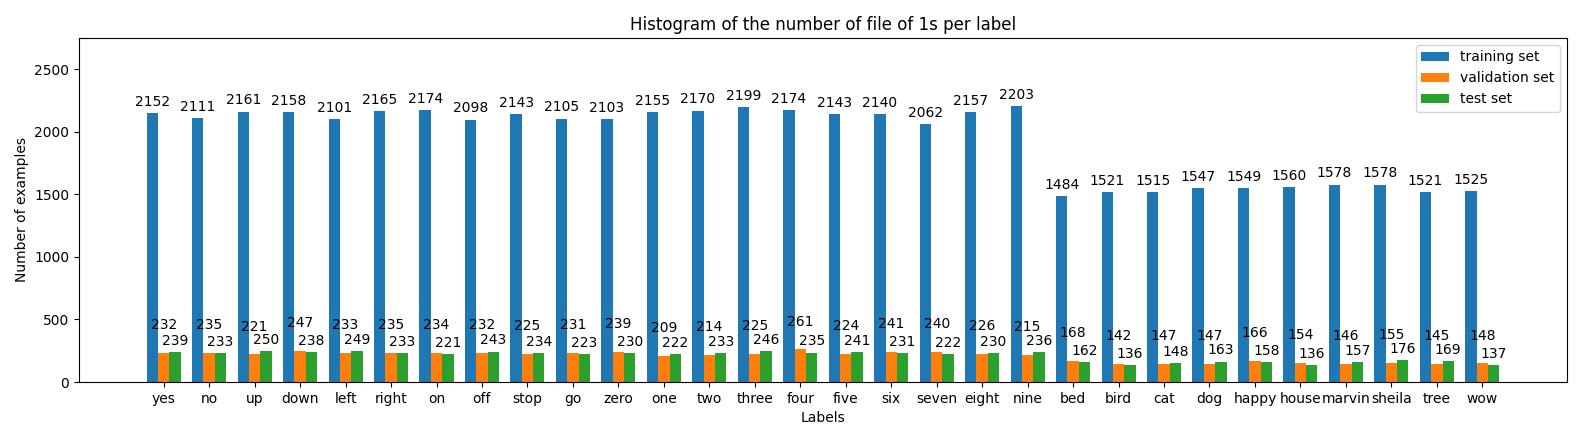
\includegraphics[width=1\textwidth]{chapters/pictures/histo_all_1s.PNG}
    \caption{Files of 1s distributions}
    \label{fig:init_dist_1s}
\end{figure}

\newpage

\section{Raw data : Does it makes sense to use them ?}

Even if audio raw files can be fed to a network and lead to a success while building really deep CNN structures, we're looking for lightweight networks and we have to highlights features to make the learning easier. Fortunately our data is relatively clean of any noise, and therefore we still can detect some patterns from the raw data. 

\begin{figure}[!h]
    \centering
    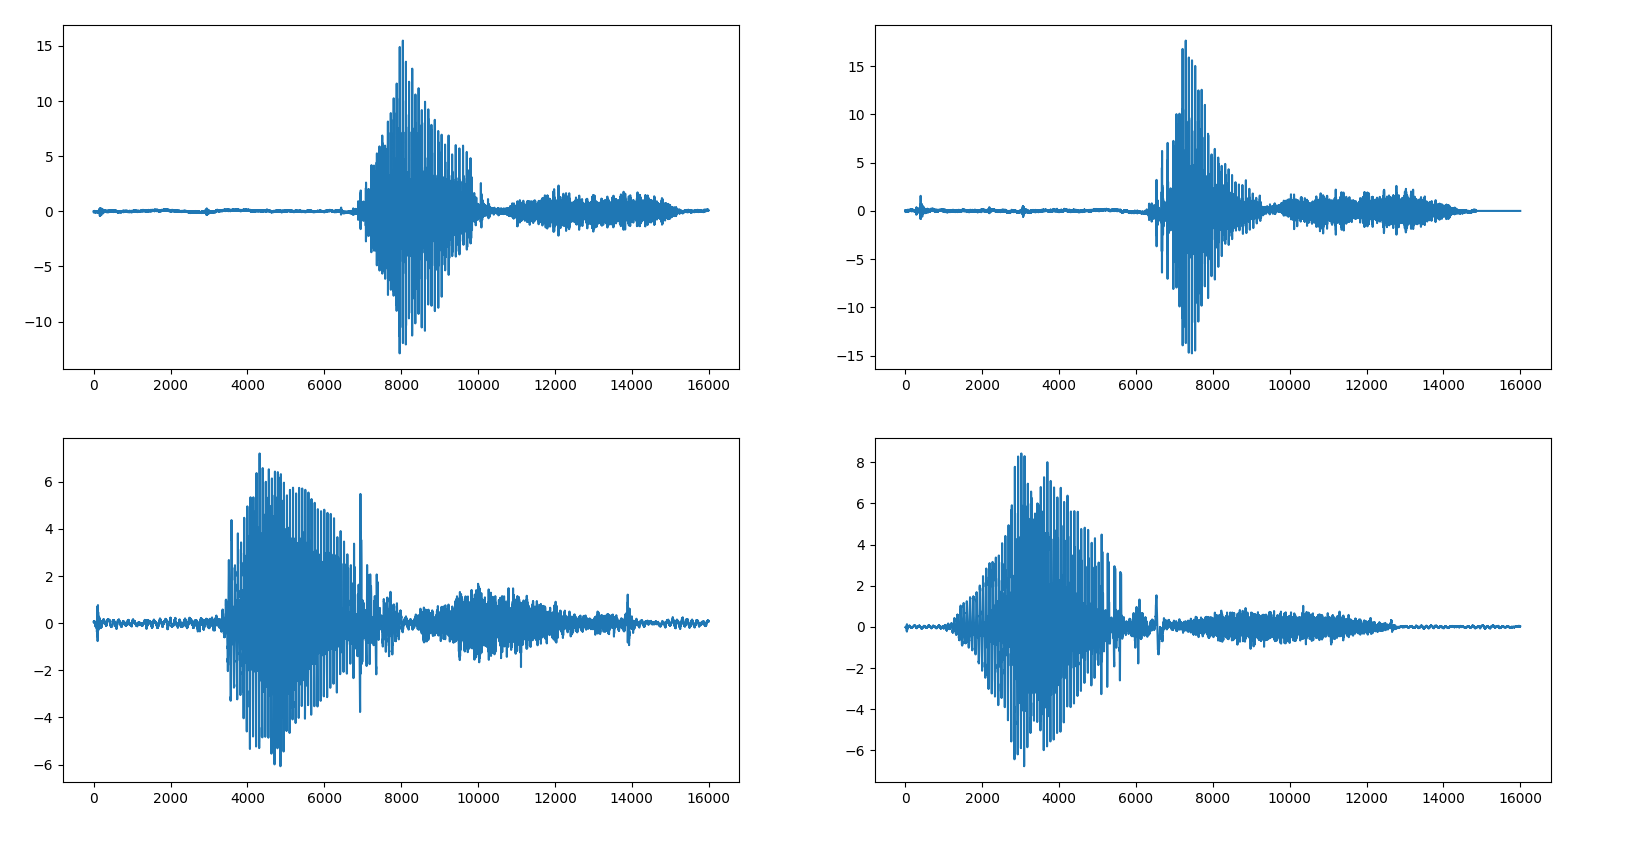
\includegraphics[width=1\textwidth]{chapters/pictures/raw_yes.PNG}
    \caption{a few examples of raw data for the word yes}
    \label{fig:raw_yes}
\end{figure}

But as we can see below, amongst the others examples you will find some that are more or less out of the pattern.


\begin{figure}[!h]
    \centering
    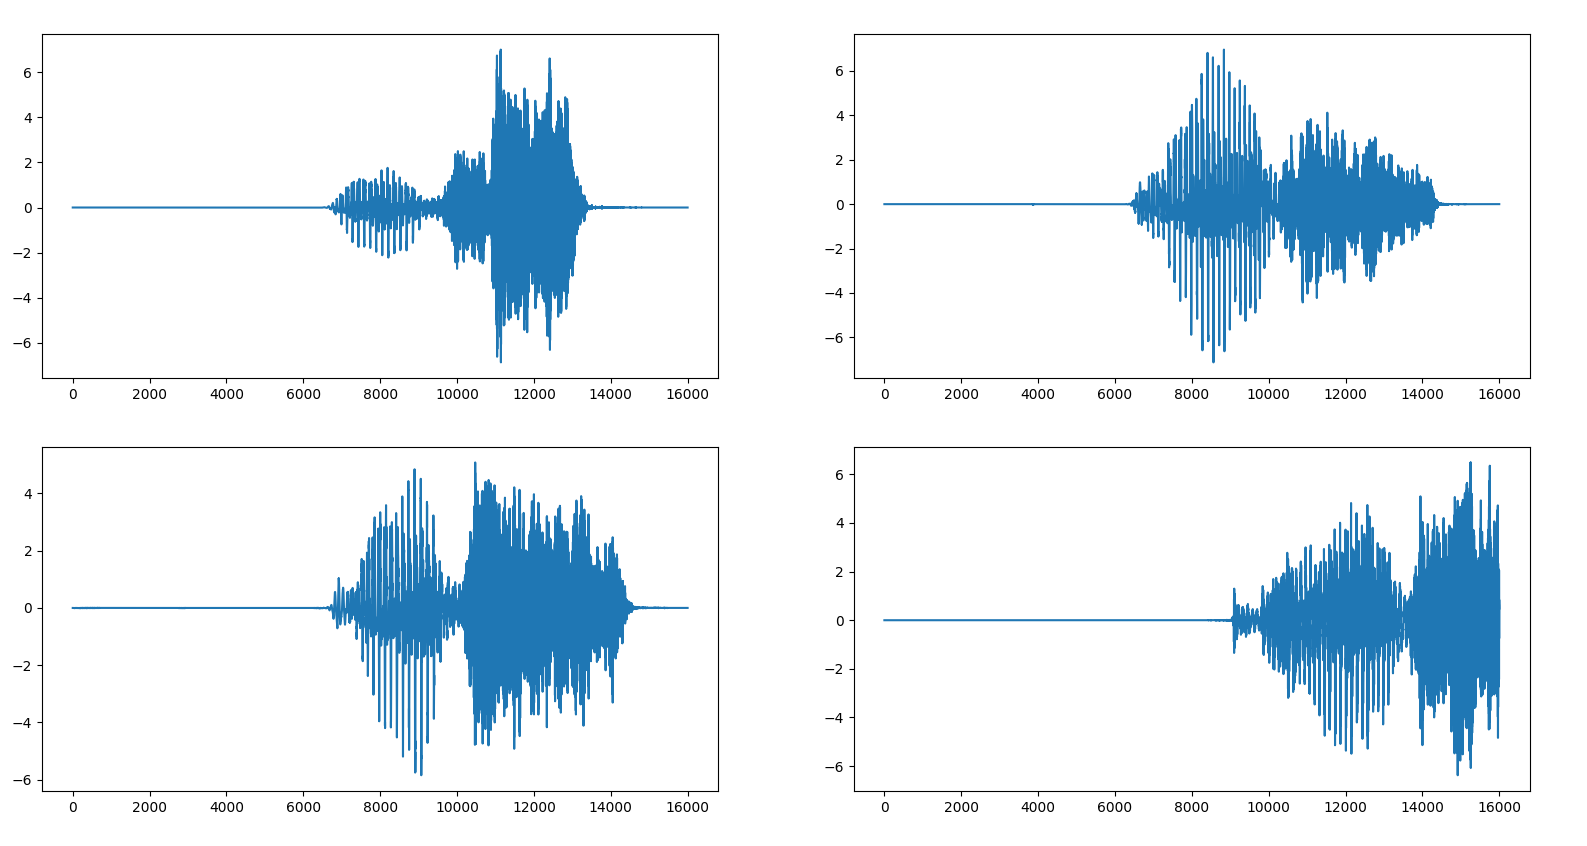
\includegraphics[width=1\textwidth]{chapters/pictures/also_yes.PNG}
    \caption{other examples of yes}
    \label{fig:also_yes}
\end{figure}


\section{Preprocessing data : Mel Frequency Cepstral Coefficients}

The mfcc features are by far the most common way to preprocess audio data \cite{review}. The idea is to represent the power spectrum in a small subset of features over time windows of the signal. The spectrum will be projected on a Mel-scale which is a way to represent the frequencies of a signal closer to how we hear sounds.

\subsection{How do we calculate those coefficients ?}

The method to calculate those coefficients has been taken from here.

\begin{itemize}
    \item The first step is to make time windows of our signal. In our case we take 30ms time windows with a 10 ms step. Which makes us 98 frames.
    \item Then we apply on each frame the discrete fourier transform to obtain an estimate of the power spectrum
    \item Then we compute the Mel-scale filterbanks and apply it the power spectrum
    \item Then we take the log of all filters from the previous step
    \item Finally, apply the discrete cosine transform to those filters
\end{itemize}

This will yields an array of $98 $ x $ n_{filters}$ , $ n_{filters}$ being an arbitrary chosen number between 10 and 40. Usually the number is 13.

\newpage

\subsection{Examples on the word yes}

\begin{figure}[!h]
    \centering
    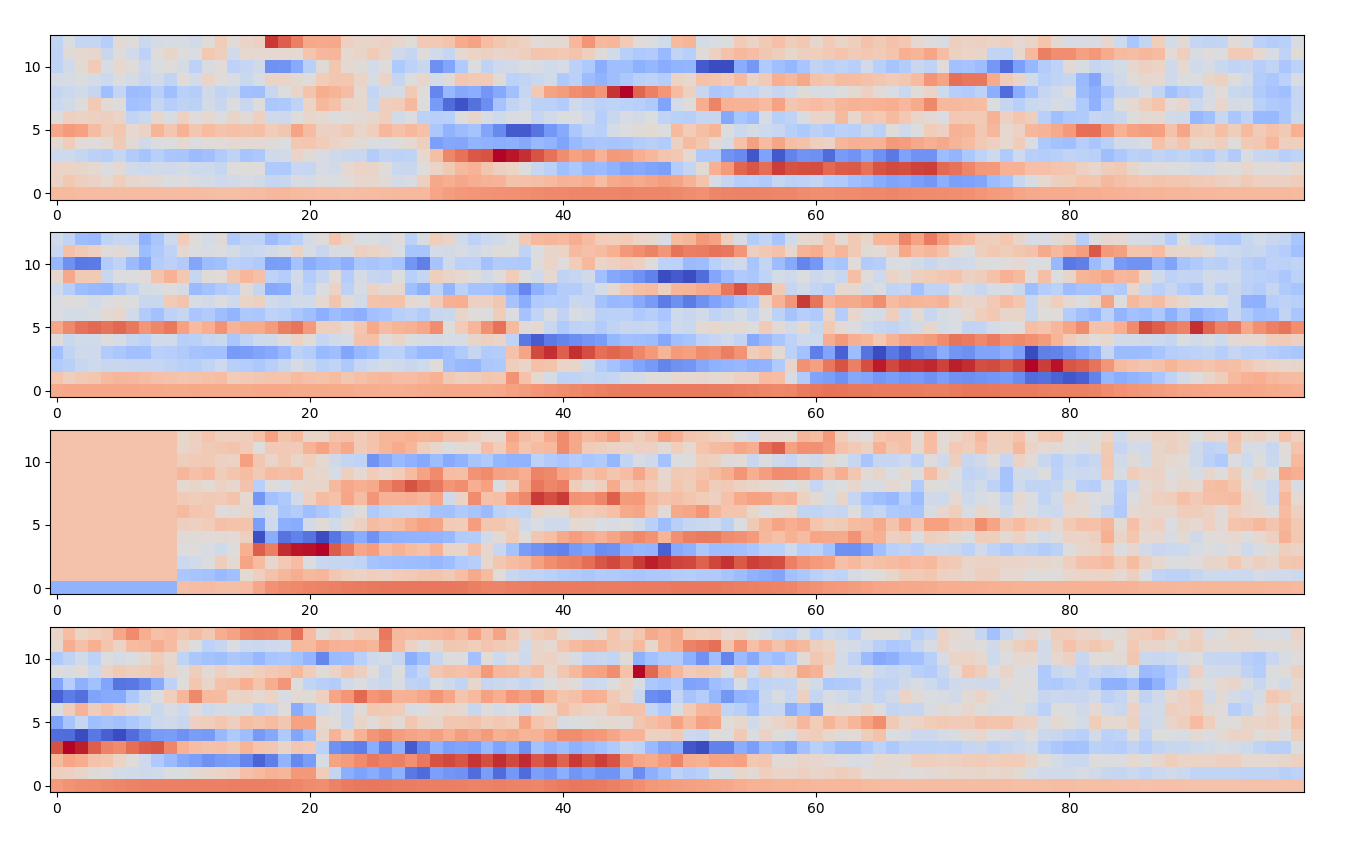
\includegraphics[width=1\textwidth]{chapters/pictures/mfcc_yes.PNG}
    \caption{examples of MFCC features on the word yes}
    \label{fig:mfcc_yes}
\end{figure}

\section{Preprocessing data : Spectral Subband centroids}

To calculate those features, you've to divide the signal into $n_sub$ subbands and take the centroid of each one. The centroid of a subband is the weighted mean of the frequencies in the signal weighted by their magnitude. The number of subbands is arbitrarly chosen (usually 26). You can see the full calculation here \cite{subband}.

\newpage

\begin{figure}[!h]
    \centering
    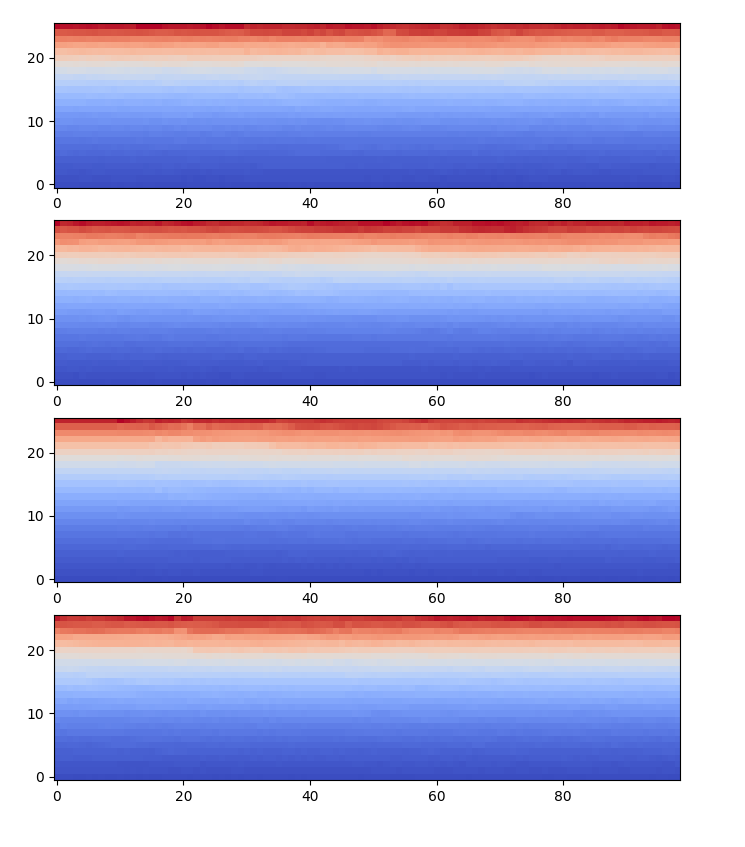
\includegraphics[width=1\textwidth]{chapters/pictures/ssc_yes.PNG}
    \caption{examples of SSC features on the word yes}
    \label{fig:mfcc_yes}
\end{figure}

Those features are extremely different from the mfcc and have been proven to be complementary \cite{subband_comp}. 